En este apartado se describirá el proceso de despliegue de la aplicación, detallando los componentes y servicios necesarios para su correcto funcionamiento. 
Se presentará un diagrama de despliegue que ilustrará la arquitectura de la aplicación y la distribución de los componentes en el entorno de ejecución. 

Como se ha visto en la sección \coloredUnderline{\hyperlink{sec:identificacion-subsistemas-analisis}{\ref*{sec:identificacion-subsistemas-analisis}. \nameref*{sec:identificacion-subsistemas-analisis}}}, la aplicación se divide en dos subsistemas principales: \textbf{restapi} y \textbf{webapp}.
El subsistema \textbf{restapi} contiene las clases que implementan la API REST y la lógica de negocio, mientras que el subsistema \textbf{webapp} abarca la interfaz de usuario de la aplicación.
Estos dos subsistemas serán desplegados en una máquina virtual de Azure, utilizando contenedores Docker para facilitar su despliegue y escalabilidad.

Para desplegar la aplicación, se han seguido los siguientes pasos:
\begin{enumerate}
    \item \textbf{Crear la máquina virtual en Azure}: Se ha creado una máquina virtual en Azure con las características mencionadas anteriormente. 
    Además, es necesario crear un grupo de recursos y una red virtual para la máquina virtual. Las características de la máquina virtual son las siguientes:
    \begin{itemize}
        \item \textbf{Sistema Operativo}: Ubuntu 20.04 LTS.
        \item \textbf{Procesador}: 2 núcleos.
        \item \textbf{Memoria RAM}: 4 GB.
        \item \textbf{Discos de datos}: 4.
        \item \textbf{E/S máxima}: 1280 MB/s.
        \item \textbf{Almacenamiento local}: 8 GB.
        \item \textbf{Red}: IP pública y DNS asociado.
    \end{itemize}

    \item \textbf{Establecer un nombre de dominio}: Se ha asociado un nombre de dominio a la dirección IP pública de la máquina virtual para facilitar el acceso a la aplicación.

    \item \textbf{Contenedores Docker}: Se ha utilizado Docker para contenerizar la aplicación y facilitar su despliegue. 
    Para facilitar la tarea se ha configurado integración continua con GitHub Actions, de forma que cada vez que se realiza un \textit{pull-request} a la rama principal del repositorio, se construyen y despliegan los contenedores en la máquina virtual de Azure.
    Se han creado dos contenedores, uno para el subsistema \textbf{restapi} y otro para el subsistema \textbf{webapp}. Cada uno de estos expone uno o varios puertos diferentes para la comunicación con el exterior.

    \item \textbf{Configuración de Nginx como Proxy Inverso}: Se ha configurado Nginx como servidor web inverso para redirigir las peticiones a los contenedores correspondientes.
    Este paso es necesario para poder garantizar la seguridad de las comunicaciones con HTTPS. La configuración de Nginx incluye:
    \begin{itemize}
        \item \textbf{Obtención de certificado SSL}: Se ha utilizado Certbot para obtener un certificado SSL gratuito de Let's Encrypt y habilitar el protocolo HTTPS en la aplicación.
        \item \textbf{Redirección de Peticiones}: Configuración de Nginx para dirigir el tráfico HTTP y HTTPS a los contenedores adecuados.
    \end{itemize}

    \item \textbf{Configuración de la base de datos}: En la aplicación se usa como base de datos Mongo DB Atlas, que es una base de datos en la nube por lo que no es necesario configurarla en la máquina virtual, 
    pero sí es necesario configurar la conexión a la base de datos en la aplicación y permitir el acceso desde la dirección IP de la máquina virtual.

    \item \textbf{Docker Compose}: Se ha utilizado Docker Compose para orquestar los contenedores de la aplicación y facilitar su despliegue en la máquina virtual de Azure.
    Se ha creado un archivo \textit{docker-compose.yml} en la máquina virtual que define los servicios de la aplicación y sus configuraciones.

\end{enumerate}

Una vez realizados estos pasos, la aplicación estará desplegada y accesible a través del nombre de dominio asociado a la dirección IP pública de la máquina virtual.
Debido a los costos asociados al uso de la máquina virtual en Azure, se ha optado por mantener la máquina virtual apagada cuando no se está utilizando la aplicación.


En la \coloredUnderline{\hyperlink{fig:6_6_Diagrama-Despliegue}{Figura \ref*{fig:6_6_Diagrama-Despliegue}: \nameref*{fig:6_6_Diagrama-Despliegue}}} se muestra el diagrama de despliegue de la aplicación.
\begin{figure}[H]
    \hypertarget{fig:6_6_Diagrama-Despliegue}{}
    \centering
    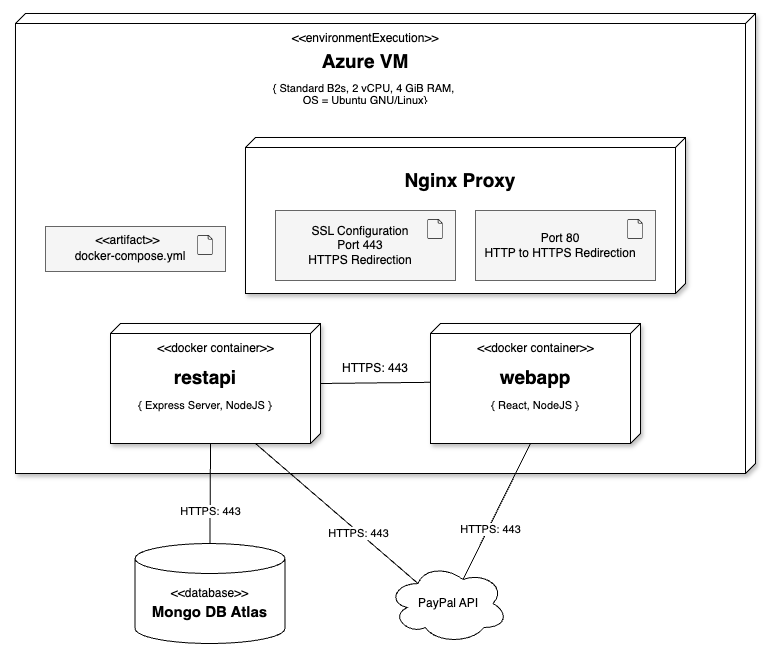
\includegraphics[width=0.8\linewidth]{figures/6-Analisis/6-Clases/6_5-Deployment.png}
    \caption{Diagrama de Despliegue de la Aplicación}
    \label{fig:6_6_Diagrama-Despliegue}
\end{figure}